\chapter{Introduction}
\label{cha:Introduction}

Autonomous vehicles used to exist solely in science fiction. In 1953, Isaac Asimov wrote Sally \citep{Asimov1953}; in 1982, Knight Rider introduced KITT \citep{Kitt1982}; but today, autonomous vehicles can be found on roads around the world. Alphabet's WAYMO is gaining traction, with cars being tested in four different US states \citep{Waymo2016}. Tesla have deployed their beta Autopilot system into all of their vehicles produced since September 2014. The system has been both hailed for saving lives and blamed for ending them \citep{TeslaHospital} \citep{TeslaUnderInvestigation}.

All of the autonomous vehicle systems currently running on public roads are designed to work alongside human driven vehicles, limiting their benefits. In order to truly embrace autonomous vehicles, we need to design systems which assume every vehicle on the road is automated. The advantages of these systems are numerous, but the most important benefit is safety.

Autonomous vehicles would be able to react to incidents much more quickly than a human driver could. A driver's 'thinking distance' often determines whether someone survives an accident or not. This distance can be greatly increased if the driver of the vehicle is under the influence of alcohol or narcotics. An autonomous vehicle would be able to react to accidents much more quickly than a human, reducing the thinking distance and improving road safety.

\begin{figure}[htb]
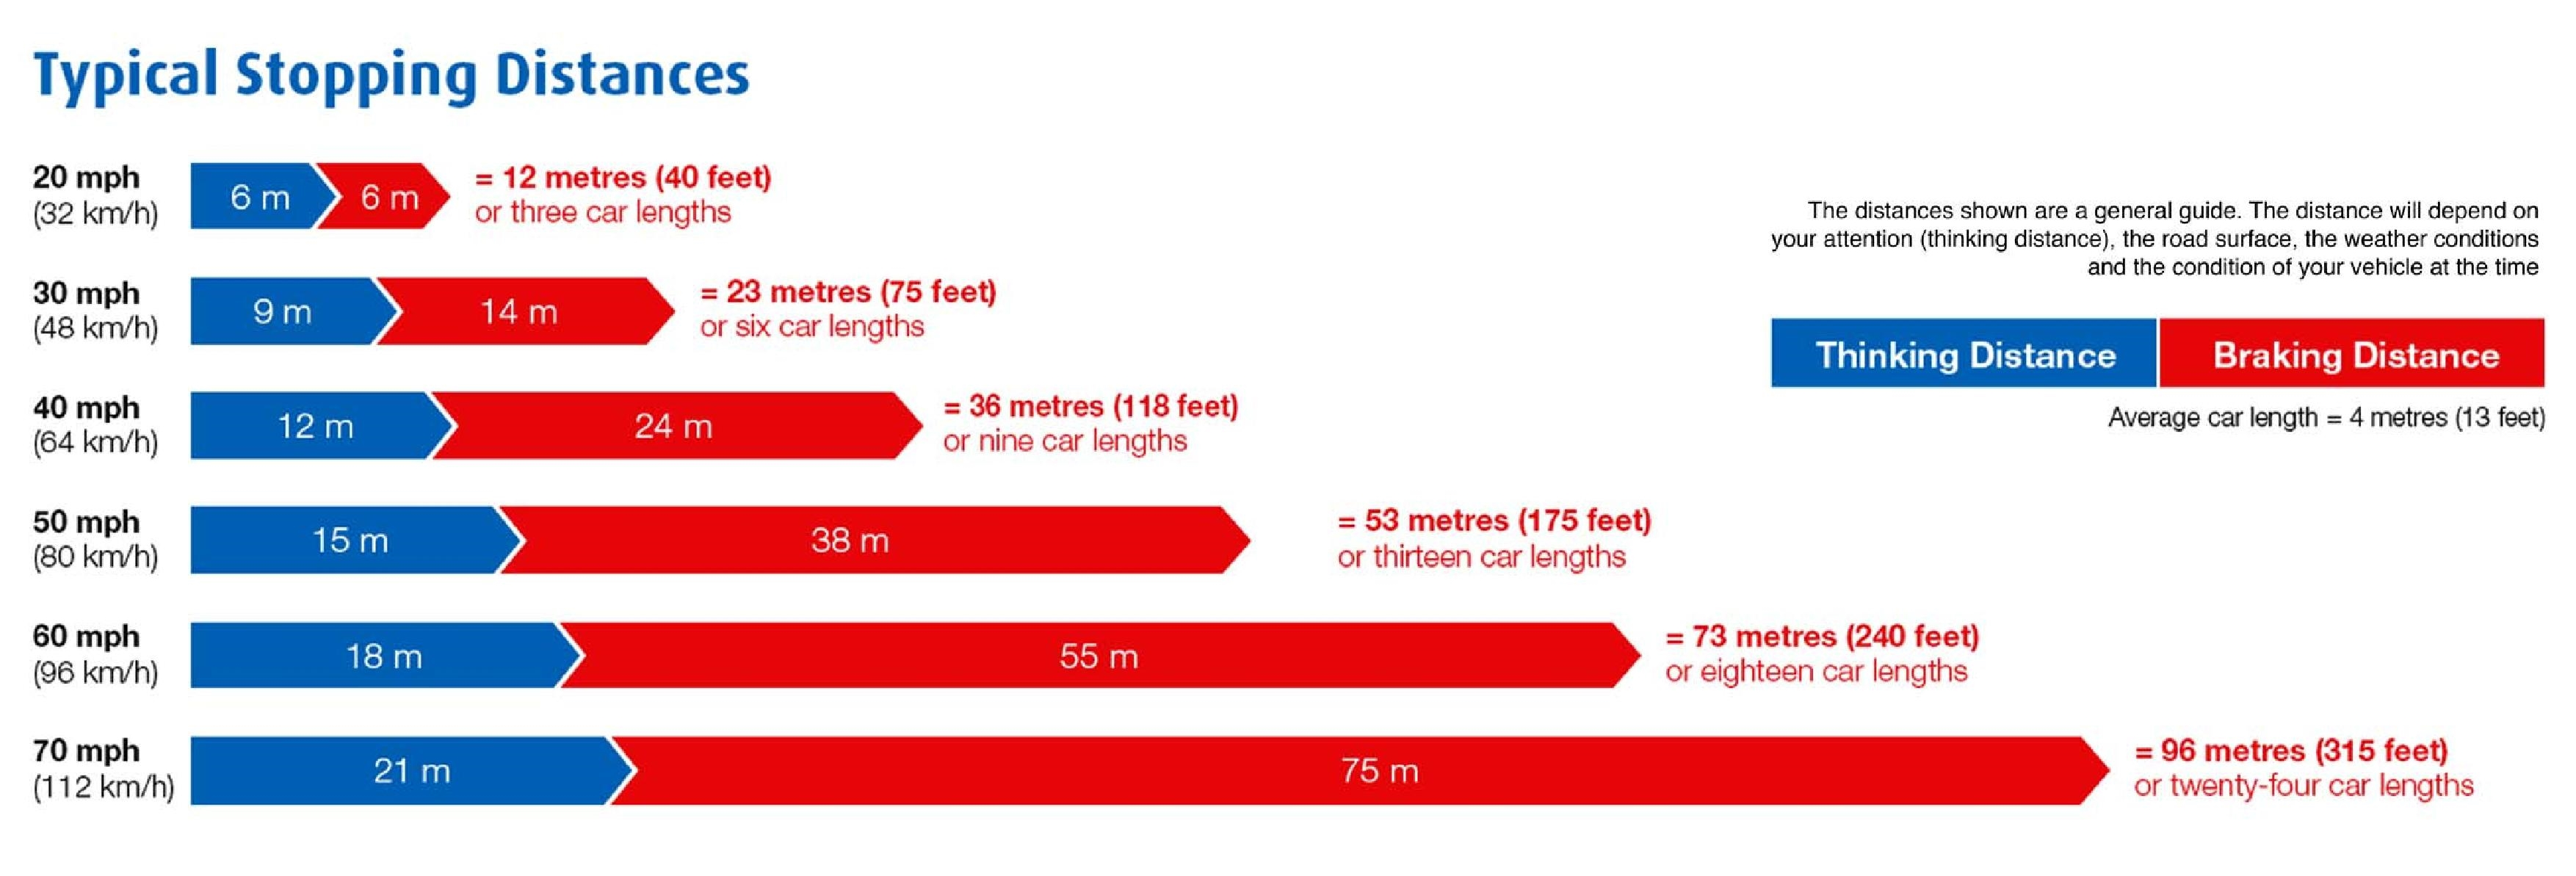
\includegraphics[width=\textwidth]{introduction/stoppingDistances.jpg}
\caption{Diagram from Rule 126 in the UK Highway Code \citep{StoppingDistances}}
\label{fig:StoppingDistances}
\end{figure}

Another benefit of autonomous vehicles is efficiency. Research by Mersky suggests that fuel conservation strategies could make autonomous vehicles up to 10\% more fuel efficient than current EPA fuel economy test results \citep{Mersky2016}. Fuel efficient vehicles are becoming increasingly important, with landmark climate change deals such as 'The Paris Agreement' introducing limits on greenhouse gas emissions globally \citep{Paris2016}. The introduction of electric vehicles into the car market is also an important factor to consider, as the driving range of such vehicles has still not managed to match that of their gasoline counterparts. Introducing efficient driving strategies through autonomous vehicles could help bring electric vehicle range up to par.

Congestion contributes to fuel loss in quite a large way. In 2014, the US wasted an estimated 3.1 billion gallons (11.7 billion litres) of fuel due to congestion \citep{Schrank2015}. Automated driving strategies, in situations such as lane changes, could reduce congestion and improve efficiency. Dangerous lane changes don't even have to result in a crash to cause delays. If a car brakes due to a dangerous merge, it can cause a ripple effect, creating a traffic jam. This ripple effect is known as a 'traffic wave' or 'traffic shock' \citep{Daganzo1994}.

As well as more quantifiable benefits, autonomous vehicles could also provide a level of comfort not currently available today. In a world where autonomous vehicles are commonplace, it is not hard to imagine people working, reading or relaxing in their car instead of focusing on driving. 

However, today there are still a number of concerns surrounding autonomous vehicles, one major issue being the reliability of the systems governing the vehicle. Systems need to be responsive and accurate. They cannot afford to fail in such safety critical environments. Today, concerns over Tesla's Autopilot system are impacting the image of the company, and the system isn't even out of beta testing yet \citep{TeslaCriticised}. 

In order to address these concerns safely, we can create simulations which test the reliability of autonomous systems. Researchers at the University of Texas set up the Autonomous Intersection Management (AIM) project, which aims to "create a scalable, safe, and efficient multiagent framework for managing autonomous vehicles at intersections" \citep{AIMProject}. The team managed to apply their simulator tested intersection software in a mixed reality test, using a real life autonomous vehicle \citep{Quinlan2010}. This demonstrates how vital simulators are when testing safety critical systems.

In this project we make a number of assumptions. Firstly we assume that the sensors resolving the positions of the vehicle and it's surrounding obstacles are perfectly accurate. We also assume that all vehicles can reliably communicate with each other and with roadside infrastructure. These assumptions ignore existing areas of research which are not considered in this paper. The focus is on how autonomous vehicles can self-organise to minimise delays in traffic, using safe and effective lane merging.

The aims of this project are as follows:
\begin{itemize}
\item Attempt to generalise the AIM codebase such that other simulators can be created for non-intersection related situations.
\begin{itemize}
\item Create a decentralised system for managing lane merging.
\item Create a centralised system for managing lane merging.
\end{itemize}
\item Compare the effectiveness of both strategies.
\end{itemize}